\chapter{Experiments on Synthetic Graphs}

The methodology described is applied to two classes of synthetic networks. These generated benchmarks allow for the comparison to the ground truth communities, and also test how well each algorithm can extract networks in increasingly difficult problem spaces.

\section{Girvan-Newmann Experiments}
The GN benchmark serves as a proving ground for an algorithm. Given its limited size, we can test a large number of parameter sets very quickly. 

%%table            parameter set 1 | parameter set 2 | parameter set 3 | parameter set 4 | parameter set  5
% mixing parameter


%% convergence curves


\begin{figure}
	\begin{tabular}{cc}
		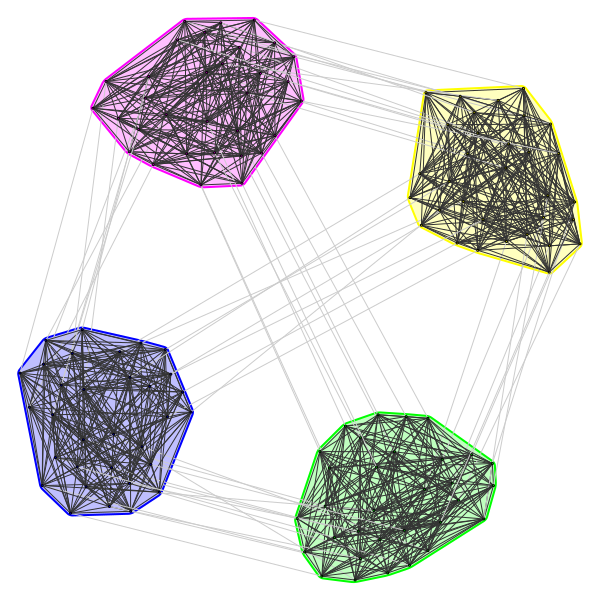
\includegraphics[width=65mm]{images/girvan_kout_1_0.png} &   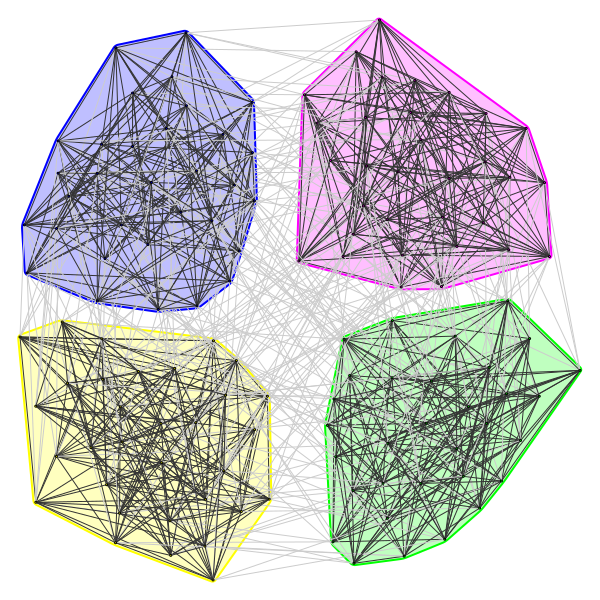
\includegraphics[width=65mm]{images/girvan_kout_4_0.png} \\
		(a) $k_{out}=1$ & (b) $k_{out}=4$ \\[6pt]
		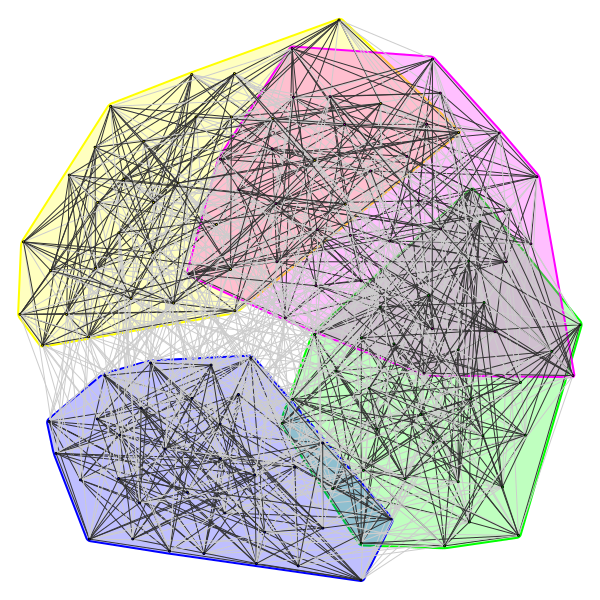
\includegraphics[width=65mm]{images/girvan_kout_7_0.png} &   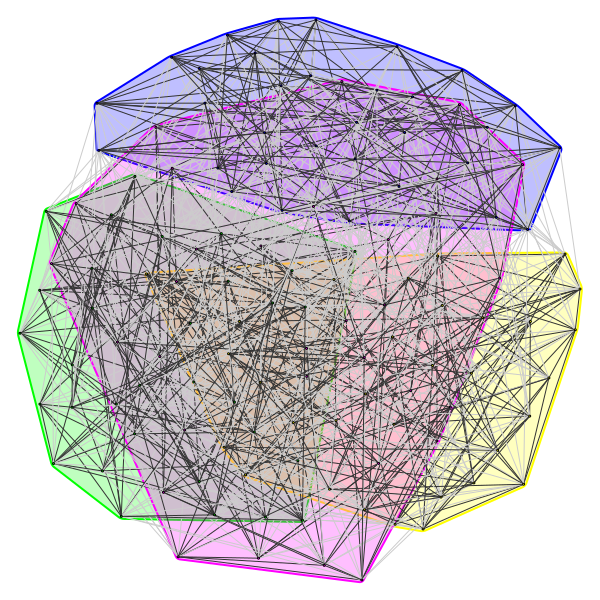
\includegraphics[width=65mm]{images/girvan_kout_8_0.png} \\
		(c) $k_{out}=7$ & (d) $k_{out}=8$ \\[6pt]
		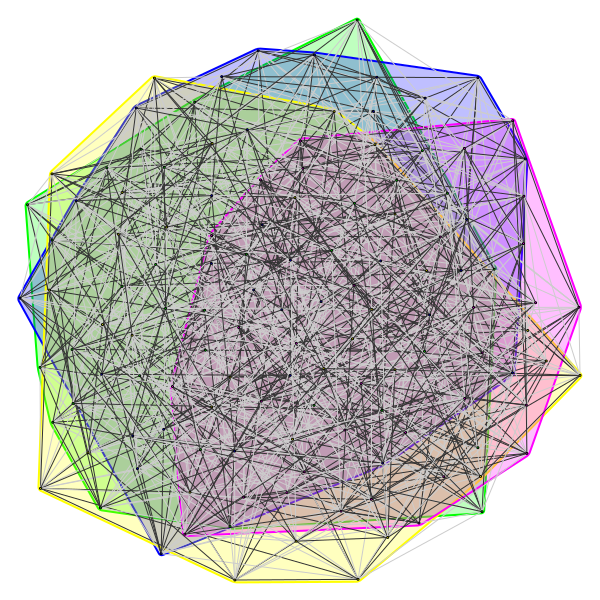
\includegraphics[width=65mm]{images/girvan_kout_9_0.png} &   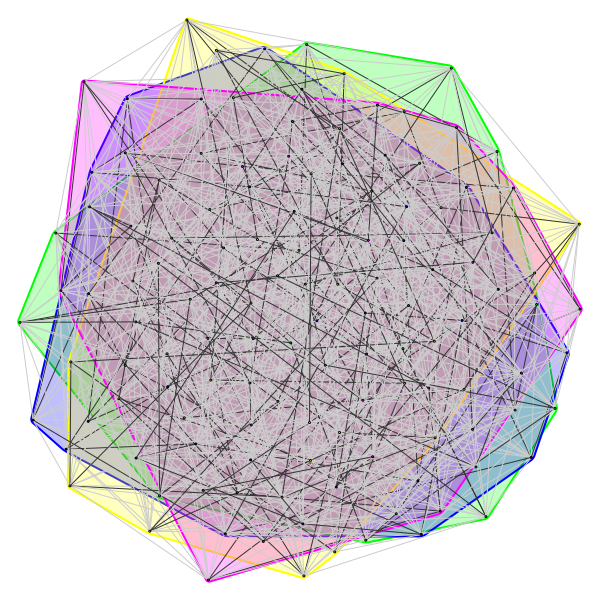
\includegraphics[width=65mm]{images/girvan_kout_13_0.png} \\
		(c) $k_{out}=9$ & (d) $k_{out}=13$ \\[6pt]
		
	\end{tabular}
	\caption{Visualizations of the GN benchmark with increasing $k_{out}$ parameters.}
\end{figure}


%% non-parametric tests

\section{LFR Benchmarks With Increasing Mixing \\ Parameter}
While the Girvan-Newmann benchmark allows for creating networks with increasingly difficult to identify communities, it is limited by its limits in terms of a fixed degree distribution, and no variance in community size. The LFR benchmark extends the planted \ell-partition model to allow a degree distribution following the power law and a mix of community sizes.

%%table            parameter set 1 | parameter set 2 | parameter set 3 | parameter set 4 | parameter set  5
% mixing parameter


%% lfr graph images


%% convergence curves


%% non-parametric tests



\section{LFR Benchmarks With Increasing Size}

%% convergence curves


%% non-parametric tests
